\documentclass[../main/main.tex]{subfiles}

\raggedbottom

\makeatletter
\renewcommand{\@chapapp}{M\'ecanique -- chapitre}
\makeatother

% \toggletrue{student}

\begin{document}
\setcounter{chapter}{1}

\chapter{Dynamique du point}

\section{Introduction}
Dans ce chapitre nous nous intéressons à étudier les causes de la mise en
mouvement d'un corps, représenté par un point matériel, et les mouvements qui en
découlent.

\subsection{Inertie et quantité de mouvement}
Mettre en mouvement un corps revient à en modifier la vitesse. Il est cependant
plus facile de mettre en mouvement (ou arrêter le mouvement) certains corps par
rapport à d'autres. Ce phénomène s'appelle l'inertie, et est
proportionnel à la masse d'un corps.

\begin{tdefi}{Définition}
    La résistance d'un corps matériel de masse $m$ à varier de vitesse est
    appelée \textbf{inertie}, quantifié par la \textbf{masse} et le
    \textbf{vecteur quantité de mouvement} du point matériel M du corps~:
    \[\boxed{\pf\Rg(\Mr) = m\vf\Rg(\Mr)}\]
    avec $\vf\Rg(\Mr)$ le vecteur vitesse du point M dans le référentiel $\Rc$.
\end{tdefi}

Il est en effet plus difficile de déplacer une voiture à l'arrêt qu'un caddie à
l'arrêt, et inversement il est plus difficile d'arrêter une voiture qu'un
caddie. Dans l'analogie électromécanique, c'est l'inductance $L$ qui s'oppose à
la variation du courant quand $m$ s'oppose à la variation de la vitesse.

\subsection{Forces fondamentales}
Les causes du mouvement d'un corps sont appelées \textbf{forces}.
\begin{tdefi}{Définition, sidebyside}
    Les \textbf{forces} caractérisent les actions mécaniques sur un point
    matériel M. Ce sont des \textbf{vecteurs} et elles sont indépendantes du
    référentiel.
    \tcblower
    L'unité d'une force est le Newton, noté N, tel que~:
    \[\boxed{\SI{1}{N} = \SI{1}{kg.m.s^{-2}}}\]
\end{tdefi}
Il existe quatre de ces forces que l'on caractérisent de «~fondamentales~», qui
permettent de classer les interactions physiques entre les systèmes~: \bigbreak
\begin{itemize}
    \item \textbf{L'interaction faible}~: elle intervient au niveau des
        \textbf{nucléons}, est de \textit{faible intensité} et de
        \underline{très courte portée} ($\approx \SI{e-18}{m}$)~;
    \item \textbf{L'interaction forte}~: responsable de la cohésion des
        \textbf{noyaux atomiques}, et permet aux protons de rester dans
        le noyau
        malgré la répulsion électromagnétique due à leurs charges électriques
        identiques. Elle est de \textit{très forte intensité} mais sur une
        \underline{très courte portée} ($\approx \SI{e-14}{m}$).
    \item \textbf{L'interaction électromagnétique}~: elle intervient entre les
        \textbf{particules chargées}, avec une \textit{forte intensité} et à
        \underline{longue portée}. Les particules de même signe se repoussent,
        tandis que celles de signes opposées s'attirent, et est responsable de
        la \textbf{cohésion des matériaux} et de leurs propriétés mécaniques
        (dureté, viscosité, propriétés chimiques…).
\end{itemize}
\begin{tprop}{Propriété}
    La force d'interaction électrostatique subie par une particule de charge
    $q_A$ de la part d'une charge $q_B$ est~: \smallbreak
    \begin{minipage}{0.45\linewidth}
        \[\Ff_{e,\rm B\ra A} = \frac{1}{4\pi\ep_0} \frac{q_Aq_B}{\rm BA^2}\uf
        \qavec
        \uf = \frac{\vv{\rm BA}}{\rm BA}\]
    \end{minipage}
    \hfill
    \begin{minipage}{0.45\linewidth}
        \begin{center}
            \includegraphics[width=\linewidth]{fe}
        \end{center}
    \end{minipage}

    \bigbreak$\uf$ est un vecteur unitaire dirigé de B vers A.
\end{tprop}
\begin{itemize}
    \item \textbf{L'interaction gravitationnelle}~: elle intervient entre les
        \textbf{particules massives} et est à \textit{faible intensité} mais à
        \ul{très longue portée}. La masse étant une grandeur positive, toutes
        les massives s'attirent entre elles. Elle prédomine à l'échelle
        astronomique et à l'origine du poids, et indirectement de la poussée
        d'\textsc{Archimède}.
\end{itemize}
\begin{tprop}{Propriété}
    La force d'interaction gravitationnelle subie par une masse
    $m_A$ de la part d'une masse $m_B$ est~: \smallbreak
    \begin{minipage}{0.45\linewidth}
        \[\Ff_{g,\rm B\ra A} = -\Gc \frac{m_Am_B}{\rm BA^2}\uf
        \qavec
        \uf = \frac{\vv{\rm BA}}{\rm BA}\]
    \end{minipage}
    \hfill
    \begin{minipage}{0.45\linewidth}
        \begin{center}
            \includegraphics[width=\linewidth]{fg}
        \end{center}
    \end{minipage}

    \bigbreak$\uf$ est un vecteur unitaire dirigé de B vers A.
\end{tprop}

\section{Les trois lois de \textsc{Newton} (1687)}
\subsection{Principe d'inertie}

\begin{tprop}
    {Première loi de \textsc{Newton}~: principe d'inertie, heart}
    Il existe des référentiels appelés \textbf{référentiels galiléens} dans lesquels un
    point matériel M soumis à \textbf{aucune action mécanique} est
    \begin{itemize}
        \item soit \textbf{au repos}~;
        \item soit en \textbf{translation rectiligne uniforme}.
    \end{itemize}
\end{tprop}

Ainsi, tout référentiel en translation rectiligne uniforme par rapport à un
référentiel galiléen est galiléen. Ils n'existent rigoureusement aucun
référentiel galiléen, mais on peut en considérer certains comme
\textit{approximativement} galiléens lorsqu'on étudie le problème sur une durée
assez courte. En reprenant les exemples du chapitre précédent~: \bigbreak
\begin{itemize}
    \item Le référentiel \textbf{héliocentrique} est supposé galiléen si le
        mouvement étudié est plus court qu'un trajet significatif du Soleil dans
        la galaxie, soit plusieurs \textbf{millions d'années}~;
    \item Le référentiel \textbf{géocentrique} est supposé galiléen si le
        mouvement étudié est plus court qu'un trajet significatif de la Terre
        autour du Soleil, soit \textbf{une année}~;
    \item Les référentiels \textbf{terrestres} sont supposés galiléens si le
        mouvement étudié est plus court qu'une rotation significative de la
        Terre, soit \textbf{une journée}.
\end{itemize}

\subsection{Principe fondamental de la dynamique}

C'est une des lois les plus importantes de la physique, permettant de relier le
mouvement cinématique (dérivée de la vitesse) d'un corps en fonction de ses
causes (les forces extérieures).

\begin{tprop}{Deuxième loi de \textsc{Newton}~: principe fondamental de la
    dynamique, heart}

    Dans un référentiel galiléen $\Rc$, la dérivée temporelle du vecteur
    quantité de mouvement $\pf\Rg(\Mr)$ d'un point matériel M de masse $m$ est
    égale à la somme des forces extérieures agissant sur le système
    $\Ff_{\ext\ra\Mr}$~:
    \[
        \boxed{\dv{\pf\Rg(\Mr)}{t} = \sum \Ff_{\ext\ra\Mr}}
    \]
    Lorsque la masse est constante, on a $\forall t$ $\pf\Rg(\Mr) =
    m\vf\Rg(\Mr)$, ainsi
    \[
        \boxed{m\af\Rg(\Mr) = \sum \Ff_{\ext\ra\Mr}}
    \]
    avec $\af\Rg(\Mr)$ le vecteur accélération du point M.
\end{tprop}

\begin{rexem}{Remarque}
    Certains mouvements ne peuvent donc pas être traités avec cette dernière
    formulation s'ils s'accompagnent d'une variation de masse~:
    \begin{itemize}
        \item Le mouvement d'une fusée qui brûle son carburant puis abandonne
            ses réservoirs~;
        \item Le mouvement d'une goutte d'eau qui s'évapore lors de sa chute.
    \end{itemize}
    Dans ces cas-là, on utilise la première formulation.
\end{rexem}

\subsection{Loi des actions réciproques}

\begin{tprop}{Troisième loi de \textsc{Newton}~: loi des actions réciproques,
    sidebyside, heart}
    Pour deux points M$_1$ et M$_2$ en interaction, la force exercée par le
    point 1 sur le point 2 est égale à l'opposé de la force exercée par le point
    2 sur le point 1~:
    \[\boxed{\Ff_{1\ra2} = - \Ff_{2\ra1}}\]
    \tcblower
    \begin{minipage}{0.45\linewidth}
        \begin{center}
            \includegraphics[height=2.6cm]{loi3a}
        \end{center}
    \end{minipage}
    \hfill
    \begin{minipage}{0.45\linewidth}
        \begin{center}
            \includegraphics[height=2.6cm]{loi3b}
        \end{center}
    \end{minipage}
\end{tprop}

\section{Ensembles de points}
Aucun système n'est rigoureusement ponctuel, mais sous certaines conditions il
est possible d'étudier le mouvement d'un corps en tant que point matériel de
manière rigoureuse. Établissons ce comportement.

\subsection{Centre d'inertie}

\begin{tdefi}{Définition}
    Le \textbf{centre d'inertie} ou \textbf{centre de gravité} G d'un ensemble
    de points matériels M$_i$ de masses $m_i$ est défini par~:
    \[\boxed{\vv{\rm OG} = \frac{1}{\sum_i m_i} \sum_i m_i \vv{{\OMr}_i}}\]
    Il s'agit du barycentre des points du système, pondéré par leur masse.
\end{tdefi}

Le centre d'inertie correspond au centre d'équilibre gravitationnel d'un
ensemble de point. Ainsi, pour mettre une règle en équilibre horizontalement il
faut la reposer en son milieu. Un marteau, en revanche, a son centre d'inertie
bien plus proche de la masse que du milieu.

Il existe une autre formulation à cette définition. En effet,
\begin{align*}
    \sum_i m_i\vv{\rm OG} &= \sum_i m_i\vv{\OMr_i}
    \\
    \Leftrightarrow
    \of &= \sum_i m_i \left( \vv{\OMr_i} - \vv{\rm OG} \right)
\end{align*}
Or, comme $\vv{\OMr_i} - \vv{\rm OG} = \vv{\rm GO} + \vv{\OMr_i} = \vv{\rm
GM_i}$, on pourra également retenir~:
\[\boxed{\sum_i m_i\vv{{\rm GM}_i} = \of}\]

\begin{rexem}{Exemple}
    Soient 2 masses $m$ placées en A et en B.
    \begin{center}
        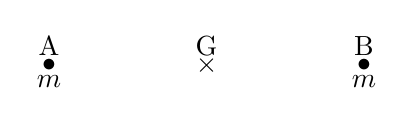
\begin{tikzpicture}[]
            \coordinate (A) at (-2,0);
            \coordinate (B) at (2,0);
            \coordinate (G) at (0,0);
            \node[] at (A) {$\bullet$};
            \node[below] at (A) {$m$};
            \node[above] at (A) {A};
            \node[] at (B) {$\bullet$};
            \node[below] at (B) {$m$};
            \node[above] at (B) {B};
            \node[] at (G) {$\times$};
            \node[above] at (G) {G};
        \end{tikzpicture}
    \end{center}
    \leftcentersright{On a~:}{$m\vv{\rm GA} + m\vv{\rm GB} = \of
    \Lra \vv{\rm GA} + \vv{\rm GB} = \of$}{car $m\neq0$}

    Or, $\vv{\rm GA} + \vv{\rm GB} = \vv{\rm GA} + \vv{\rm GA} + \vv{\rm AB}$,
    donc
    \begin{align*}
        2\vv{\rm GA} + \vv{\rm AB} &= \of
        \\
        \Lra
        2\vv{\rm AG} &= \vv{\AB}
        \\
        \Lra
        \Aboxed{\vv{\rm AG} &= \frac{1}{2}\vv{\rm AB}}
    \end{align*}
    Avec $3m$ en A et $m$ en B~:
    \begin{center}
        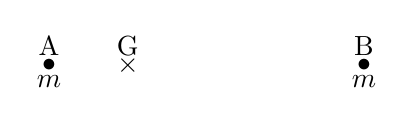
\begin{tikzpicture}[]
            \coordinate (A) at (-2,0);
            \coordinate (B) at (2,0);
            \coordinate (G) at (-1,0);
            \node[] at (A) {$\bullet$};
            \node[below] at (A) {$m$};
            \node[above] at (A) {A};
            \node[] at (B) {$\bullet$};
            \node[below] at (B) {$m$};
            \node[above] at (B) {B};
            \node[] at (G) {$\times$};
            \node[above] at (G) {G};
        \end{tikzpicture}
    \end{center}
    \leftcentersright{Cette fois,}{$3m\vv{\rm GA} + m\vv{\rm GB} = \of
    \Lra 3\vv{\rm GA} + \vv{\rm GB} = \of$}{car $m\neq0$}

    Or, $3\vv{\rm GA} + \vv{\rm GB} = 3\vv{\rm GA} + \vv{\rm GA} + \vv{\rm AB}$,
    donc
    \begin{align*}
        4\vv{\rm GA} + \vv{\AB} &= \of
        \\
        \Lra
        4\vv{\rm AG} &= \vv{\AB}
        \\
        \Lra
        \Aboxed{\vv{\rm AG} &= \frac{1}{4}\vv{\rm AB}}
    \end{align*}
\end{rexem}

Cette définition peut être étendue aux solides qui peuvent être vus comme un
ensemble infini de points infiniment proches. Dans ce cas, la somme discrète
devient une intégrale.

\subsection{Quantité de mouvement d'un ensemble de points}

On souhaiterait pouvoir étudier un ensemble de points comme le mouvement d'un
point unique, comme le centre d'inertie. Pour cela, il faut étudier la quantité
de mouvement d'un ensemble de points.

\begin{tdefi}{Définition}
    Le vecteur quantité de mouvement d'un ensemble $\Sc$ de points matériels
    M$_i$ de masses $m_i$ est défini par~:
    \[\boxed{\pf(\Sc) = \sum_i m_i \vf(\Mr_i)}\]
\end{tdefi}

Pour que les choses soient simples, il faudrait donc que $\pf(\Sc)$ soit relié
au centre d'inertie. Or,

\[
    \vf(\Gr) = \dv{\rm OG}{t} = \frac{1}{\sum_i m_i} \underbrace{\sum_i m_i
    \dv{{\OMr}_i}{t}}_{\pf(\Sc)}
    \Lra
    \boxed{\pf(\Sc) = m_{\tot}\vf(\Gr)}
\]

\begin{bror}{\includehand{-90}{0.8cm}}
    \centering\bfseries
    La quantité de mouvement d'un ensemble de points est la quantité de
    mouvement d'un point matériel placé en $G$ et de masse $m_{\tot}$~: tout se
    passe comme si la masse était concentrée en G.
\end{bror}

\subsection{Théorème de la résultante cinétique}
Si on peut étudier la cinématique d'un corps par l'étude de son centre de
gravité, comment les forces interviennent-elles sur cet ensemble de points~?
Considérons pour simplifier un système de deux points M$_1$ et M$_2$ de masses
$m_1$ et $m_2$ en mouvement dans un référentiel galiléen. On peut appliquer le
principe fondamental de la dynamique à chacun d'entre eux~:
\[\dv{\pf(\Mr_1)}{t} = \Ff_{\Mr_2\ra\Mr_1} + \Ff_{\ext\ra\Mr_1}\]
avec deux types de forces~: les forces intérieures du système, ici celles
exercées par M$_2$ sur M$_1$, et les forces extérieures, c'est-à-dire toutes les
autres. En faisant de même pour M$_2$~:
\[\dv{\pf(\Mr_2)}{t} = \Ff_{\Mr_1\ra\Mr_2} + \Ff_{\ext\ra\Mr_2}\]
Ainsi, avec la définition de la quantité de mouvement d'un ensemble de points,
\[\dv{\pf(\Sc)}{t} = \underbrace{\Ff_{\Mr_1\ra\Mr_2}+\Ff_{\Mr_2\ra\Mr_1}}_{= \of
\text{ d'après la 3ème loi}} + \Ff_{\ext\ra\Mr_1} + \Ff_{\ext\ra\Mr_2}\]
\begin{tprop}{Théorème de la résultante cinétique}
    Le principe fondamental de la dynamique pour un point matériel s'applique à
    un ensemble de point en prenant pour point matériel le centre d'inertie G
    affecté de la masse totale $m_{\tot}$ du système, en ne considérant que les forces
    extérieurs s'appliquant à l'ensemble~:
    \[\boxed{m_{\tot}\dv{\vf(\Gr)}{t} = \sum \Ff_{\ext}}\]
\end{tprop}

\begin{tror}{, hand}
    Le mouvement du centre de gravité n’est affecté que par les forces
    extérieures au système. Ainsi, dans la suite, on étudiera le mouvement du
    centre de gravité, de masse $m_{\tot}$, soumis aux forces extérieures au
    système.
\end{tror}

\section{Méthode générale de résolution en mécanique}
\begin{enumerate}[label=\sqenumi]
    \litem{De quoi parle-t-on~?} Quel est l'objet en mouvement, dans quel
    référentiel étudie-t-on le mouvement~?

    \litem{Schéma.} Faire un schéma du problème dans une situation quelconque.

    \litem{Modélisation.} Donner le repère, les origines spatiale et temporelle,
    les représenter sur le schéma et \textit{définir les notations} nécessaires.

    \litem{Bilan des forces.} Faire le bilan des forces, les exprimer dans le
    repère choisi et les représenter sur le schéma.

    \litem{Deuxième loi de \textsc{Newton}.} Appliquer le PFD au système.

    \litem{Équations scalaires.} Donner les trois équations $\ddot{x}$,
    $\ddot{y}$ et $\ddot{z}$.

    \litem{Répondre aux questions.} Le plus souvent, obtenir les équations
    horaires $x(t)$, $y(t)$ et $z(t)$.
\end{enumerate}

\begin{instruc}[trans]{Transition}
    Avec ces outils, voyons maintenant quelques forces et situations usuelles
    que l'on rencontrera en dynamique.
\end{instruc}

\section{Le poids}
\subsection{Définition}

\begin{tdefi}{Définition}
    Dû à l'attraction gravitationnelle de la Terre, un corps de masse $m$ à sa
    surface subit une force que l'on appelle le \textbf{poids}, telle que~:
    \[\boxed{\Pf = m\gf = -mg\uz}\]
    avec $\gf$ le vecteur \textbf{accélération de la pesanteur}, de norme $g =
    \norm{\gf} = \SI{9.81}{m.s^{-2}}$ et dirigé verticalement vers le sol. Par
    définition de l'interaction gravitationnelle, on a
    \[\gf = -\Gc \frac{m_T}{R_T{}^2}\uz\]
    avec $m_T$ et $R_T$ la masse et le rayon de la Terre, $\Gc$ la constante
    gravitationnelle, et $\uz$ vertical ascendant.
\end{tdefi}

\subsection{La chute libre}
\begin{rdefi}{Déf.}
    Un système en chute libre pure ne subit que l'action de son poids.
\end{rdefi}

\hspace*{-.75cm}
\begin{minipage}{0.65\linewidth}
    \begin{enumerate}[label=\sqenumi]
        \litem{De quoi parle-t-on~?} Le mouvement d'une balle lancée avec un
            vecteur vitesse initiale $\vfo$ dans le référentiel du laboratoire.
        \litem{Schéma}. \bigbreak
    \end{enumerate}
\end{minipage}
\hfill
\begin{minipage}{0.30\linewidth}
    \begin{center}
        \includegraphics[width=\linewidth]{cl_ssf}
    \end{center}
\end{minipage}
\begin{enumerate}[label=\sqenumi, start=3]
    \litem{Modélisation}.
        \begin{itemize}
            \item On suit la trajectoire du centre d'inertie de la balle par le
                point matériel M de masse $m$.
            \item Repère~: $y$ verticale ascendantes, $x$ direction du lancer,
                $z$ tel que $(\ux, \uy, \uz)$ soit une base orthonormée directe
                (BOND).
            \item Instant initial~: moment où la balle est lancée.
            \item Origine spatiale~: position de la balle à l'instant initial
                ($\OM(0) = \of$).
            \item On note $\alpha$ l'angle du vecteur $\vfo$ avec l'axe
                horizontal et $v_0$ sa norme, tel que
                \[\vf(0) = v_0\cos\alpha\ux + v_0\sin\alpha\uy\]
        \end{itemize}
    \litem{Bilan des forces.} Ici, seul le poids s'applique~:
        \[
            \begin{array}{ll}
                \textbf{Poids} & \Pf = m\gf = -mg\uy
            \end{array}
        \]
    \item \leftcenters{\textbf{PFD.}}{$m\af = \Pf$}
    \litem{Équations scalaires.} On projette sur les axes~:
        \[
            \left\{
                \begin{array}{l}
                    m\ddot{x}(t) = 0\\
                    m\ddot{x}(t) = -mg\\
                    m\ddot{x}(t) = 0
                \end{array}
            \right.
        \]
        On s'intéresse au mouvement plan donc pas à la coordonnée $z$. Aussi, la
        masse n'étant pas nulle, elle se simplifie dans les équations et on a
        \[
            \left\{ 
                \begin{array}{l}
                    \ddot{x}(t) = 0\\
                    \ddot{y}(t) = -g
                \end{array}
            \right.
        \]
        On remarque que l'accélération ne dépend pas de la masse.
\end{enumerate}
\begin{tror}{, hand}
    Lors d’une chute libre sans frottements, la masse du corps en chute
    n’intervient pas. Cela signifie en particulier que, dans le vide, tous les
    corps chutent à la même
    vitesse.\footnote{\url{https://www.youtube.com/watch?v=E43-CfukEgs}}
\end{tror}
\begin{enumerate}[resume, label=\sqenumi]
    \litem{Répondre aux questions.}
        On intègre l'accélération pour obtenir la vitesse~:
        \[
            \left\{
                \begin{array}{l}
                    \dot{x}(t) = K_1\\
                    \dot{y}(t) = -gt + K_2
                \end{array}
            \right.
            \qor
            \left\{
                \begin{array}{l}
                    \dot{x}(0) = v_0\cos\alpha = K_1\\
                    \dot{y}(0) = v_0\sin\alpha = K_2
                \end{array}
            \right.
            \Ra
            \boxed{
            \left\{
                \begin{array}{l}
                    \dot{x}(t) = v_0\cos\alpha\\
                    \dot{y}(t) = -gt + v_0\sin\alpha
                \end{array}
            \right.
            }
        \]
        De même pour les équations horaires du mouvement~:
        \[
            \left\{
                \begin{array}{l}
                    x(t) = v_0t\cos\alpha + C_1\\
                    y(t) = \DS -\frac{1}{2}gt^2 + v_0t\sin\alpha + C_2
                \end{array}
            \right.
            \qor
            \left\{
                \begin{array}{l}
                    x(0) = 0 = C_1\\
                    y(0) = 0 = C_2
                \end{array}
            \right.
            \Ra
            \boxed{
            \left\{
                \begin{array}{l}
                    x(t) = v_0t\cos\alpha\\
                    y(t) = \DS -\frac{1}{2}gt^2 + v_0t\sin\alpha
                \end{array}
            \right.
            }
        \]
\end{enumerate}
Si on cherche la trajectoire, il s'agit alors d'obtenir la courbe $y(x)$ décrite
dans le plan $xy$, c'est-à-dire éliminer le temps $t$. À partir de l'équation
horaire sur $\ux$, on a
\begin{gather*}
    t = \frac{x}{v_0\cos\alpha}\\
    \Ra
    y(x) = - \frac{1}{2}g \frac{x^2}{v_0{}^2\cos^2\alpha} + v_0\sin\alpha
    \frac{x}{v_0\cos\alpha}
    \\
    \Lra
    \boxed{y(x) = - \frac{g}{2v_0{}^2\cos^2\alpha}x^2 + x\tan\alpha}
\end{gather*}
C'est une parabole~:

\begin{center}
    \includegraphics[width=.7\linewidth]{cl_ssf-traj}
\end{center}

On peut en définir deux caractéristiques principales, la \textbf{porté} et la
\textbf{flèche}.

\begin{tdefi}{Définition~: portée d'un tir}
    La \textbf{portée} d'un tir est la distance \textbf{horizontale} entre
    l'origine du tir et l'endroit où retombe le tir.
\end{tdefi}

Autrement dit, on trouve $x_P$ tel que~:
\begin{gather*}
    y(x_P) = 0
    \\
    \Lra
    x_P\left(- \frac{g}{2v_0{}^2\cos^2\alpha}x_P + \tan\alpha\right) = 0
\end{gather*}
On cherche $x_P \neq 0$ (origine du tir), d'où
\begin{gather*}
    - \frac{g}{2v_0{}^2\cos^2\alpha}x_P + \tan\alpha = 0
    \\
    \Lra
    x_P = \frac{2v_0{}^2\cos^2\alpha}{g}\tan\alpha =
    \frac{2v_0{}^2\cos^{\cancel{2}}\alpha}{g}
    \frac{\sin\alpha}{\cancel{\cos\alpha}}
    \\
    \Lra
    \boxed{x_P = \frac{v_0{}^2}{g}\times 2\sin\alpha\cos\a =
    \frac{v_0{}^2}{g}\sin(2\a)}
\end{gather*}
Ainsi, \underline{pour un tir à altitude nulle}, la portée est maximale si
$\sin(2\a) = 1$, soit \fbox{$\a = \pi/4$}.

\begin{tdefi}{Définition~: flèche d'un tir}
    La \textbf{flèche} d'un tir est la \textbf{hauteur maximale} atteinte par le
    projectile.
\end{tdefi}

On trouve $y_F$ quand la vitesse \textbf{verticale} s'annule, $\dot{y} = 0$~;
ainsi
\begin{gather*}
    -gt_F + v_0\sin\alpha=0
    \Lra
    t_F = \frac{v_0\sin\a}{g}\\
    \Ra
    y_F = y(t_F) = -\frac{1}{2}g \left( \frac{v_0\sin\a}{g} \right)^2 +
    v_0\sin\a\times \frac{v_0\sin\a}{g}
    \\
    \Lra
    \boxed{y_F = \frac{v_0{}^2}{2g}\sin^2\alpha}
\end{gather*}
Le maximum se trouve en $\a = \pi/2$.

\begin{rexem}{Exercice}
    Pour quel angle le temps de vol est-il le plus grand~?
    \tcblower
    %\cswitch{white}{
    Le temps de vol correspond au temps pour lequel le projectile retombe au
    sol, c'est-à-dire $t(x_P)$. \smallbreak
    \leftcenters{Ainsi,}{
        $%\DS
        t_{\max} = t(x_P)
        \Lra
        t_{\max} = \frac{\frac{v_0{}^{\cancel{2}}}{g}\times
            2\sin\a\bcancel{\cos\a}}{\cancel{v_0}\bcancel{\cos\a}}
        \Lra
        \boxed{t_{\max} = 2 \frac{v_0}{g}\sin\a}$} \smallbreak
    Le temps de vol est donc maximal pour $\alpha = \pi/2$.%}
\end{rexem}

\section{Poussée d'\textsc{Archimède}}
\begin{tdefi}{Définition}
    Lorsqu'un objet est dans un fluide, il subit une force nommée
    \textbf{poussée d'\textsc{Archimède}} et égale à l'opposé du poids du fluide
    déplacé. Elle est parfois notée $\Pif$ ou $\Ff_A$, et on a~:
    \[\boxed{\Ff_A = -\rho\ind{fluide}V\ind{immergé}\gf}\]
    avec $\rho\ind{fluide}$ la masse volumique du fluide et $V\ind{immergé}$ le
    volume de l'objet qui est dans le fluide.
\end{tdefi}

\begin{rexem}{Exercice}
    Quelle est la proportion immergée d'un glaçon~? On donne $\rho\ind{eau} =
    \SI{1.00e3}{kg.m^{-3}}$ et $\rho\ind{glace} = \SI{9.17e2}{kg.m^{-3}}$.
    \tcblower
    %\cswitch{white}{
    \begin{minipage}{0.75\linewidth}
        On suppose un glaçon immobile partiellement plongé dans de l'eau à
        la surface de la Terre. \bigbreak

        Ce glaçon subit son poids et la poussée d'\textsc{Archimède}, et a
        une accélération nulle car immobile, donc avec le PFD~:
        \begin{gather*}
            \of = \Ff_A + \Pf
        \end{gather*}
    \end{minipage}
    \hfill
    \begin{minipage}{0.20\linewidth}
        \begin{center}
            \includegraphics[width=\linewidth]{glacon}
        \end{center}
    \end{minipage}

    Or,
    \begin{gather*}
        \Pf = m\gf = \rho\ind{glace}V\ind{glaçon}\gf
        \qet
        \Ff_A = -\rho\ind{eau}V\ind{immergé}\gf
    \end{gather*}
    D'où
    \begin{gather*}
        -\rho\ind{eau}V\ind{immergé}\cancel{\gf} +
        \rho\ind{glace}V\ind{glaçon}\cancel{\gf}
        \\\Lra
        \boxed{\frac{V\ind{immergé}}{V\ind{glaçon}} =
        \frac{\rho\ind{glace}}{\rho\ind{eau}} = \SI{91.7}{\%}}
    \end{gather*}
    On observe également qu'un objet \textbf{plus dense} que le fluide aura
    une proportion immergée $> 1$~: il ne sera donc pas à l'équilibre
    mécanique et coulera.
%}
\end{rexem}

\section{Frottements fluides}
\subsection{Force de frottement fluide}
\begin{tdefi}{Définition}
    Un objet en mouvement dans un fluide subit une force de frottements dite
    fluide $\Ff_f$ qui est une force de freinage, donc opposée à la
    direction de la vitesse $\vf$. Selon la norme de la vitesse, on a~:
    \bigbreak

    \begin{minipage}{0.45\linewidth}
        \begin{itemize}
            \item Pour les \textbf{faibles vitesses}, elle est
                \textbf{proportionnelle} à $v$~:
                \[\boxed{\Ff_f = -\a\vf}\]
                %avec $\a$ en \si{kg.s^{-1}}.
        \end{itemize}
    \end{minipage}
    \begin{minipage}{0.45\linewidth}
        \begin{itemize}
            \item Pour les \textbf{vitesses élevées}, elle est
                \textbf{quadratique} avec $v$~:
                \[\boxed{\Ff_f = -\beta v\vf}\]
                %avec $\beta$ en \si{kg.m^{-1}}.
        \end{itemize}
    \end{minipage}
\end{tdefi}

\begin{rrema}{Remarque}
    En pratique, on verra souvent
    \[\beta = \frac{1}{2}\rho\ind{fluide}Sc_x\]
    avec $\rho\ind{fluide}$ la masse volumique du fluide, $S$ la surface
    frontale («~l'ombre~» que fait l'objet sur un flux), et $c_x$ un coefficient
    sans dimension dépendant surtout de la forme de l'objet.
\end{rrema}

\subsection{Chute libre sans vitesse initiale avec frottements linéaires}
\hspace*{-0.75cm}
\begin{minipage}{0.65\linewidth}
    \begin{enumerate}[label=\sqenumi]
        \litem{De quoi parle-t-on~?} Le mouvement d'une bille lâchée dans une
            éprouvette d'huile dans le référentiel de la salle de TP.
        \litem{Schéma}.
    \end{enumerate}
\end{minipage}
\hfill
\begin{minipage}{0.30\linewidth}
    \begin{center}
        \includegraphics[height=4cm]{cl_fl}
    \end{center}
\end{minipage}
    \begin{enumerate}[label=\sqenumi, start=3]
        \litem{Modélisation.}
            \begin{itemize}
                \item On repère la bille par la position de son centre d’inertie M.
                \item Repère : $y$ est la verticale ascendante, $x$ et $z$ sont deux
                    vecteurs horizontaux tels que $\ux, \uy, \uz$ soit une base
                    orthonormale directe (BOND).
                \item Instant initial : le moment où la bille entre dans le
                    glycérol.
                \item Origine : la position de la bille à son entrée dans le
                    glycérol.
                \item On néglige pour simplifier la poussée d’\textbf{Archimède}.
                \item On note $m$ sa masse, $\alpha$ le coefficient de frottement et
                    $\gf$ l’accélération de la pesanteur.
            \end{itemize}
    \litem{Bilan des forces.}
        \[
            \begin{array}{ll}
                \textbf{Poids} & \Pf = m\gf = -mg\uy\\
                \textbf{Frottements fluide} & \Ff_f = -\a\vf = -\a\dot{y}\uy
            \end{array}
        \]
    \item \leftcenters{\textbf{PFD.}}{$m\af = \Pf + \Ff$}
    \litem{Équations scalaires}.
        \[
            \left\{
                \begin{array}{rcl}
                    m\xpp(t) & = & -\a\xp\\
                    m\ypp(t) & = & -\a\yp - mg\\
                    m\zpp(t) & = & -\a\zp
                \end{array}
            \right.
        \]
    \litem{Répondre aux questions.} On obtient ici trois équations
        différentielles sur la vitesse ($v_x = \xp$, $v_y = \yp$ et $v_z =
        \zp$), mais en absence de vitesse initiale sur $v_x$ et $v_z$, il n'y
        aura pas de mouvement sur ces coordonnées~: on s'intéresse donc à
        l'équation différentielle sur $v_y$ que l'on appelle simplement $v$,
        avec $\tau = m/\a$~:
        \[\boxed{\dv{v}{t} + \frac{\alpha}{m}v = -g}
        \Lra
        \dv{v}{t} + \frac{v}{\tau} = -g\]
\end{enumerate}

Une résolution complète demande de discerner solution homogène et particulière
puis d'utiliser les conditions initiales, pour trouver
\[v(t) = g\tau\left(\exr^{-t/\tau}-1\right)\]

On peut développer une autre approche générique pour obtenir des grandeurs
typiques d'un système à partir de l'équation différentielle qui régit son
fonctionnement~: l'\textbf{adimensionnement}. \bigbreak

On définit $v^* = v/V$, $t^* = t/T$ avec $V$ et $T$ des constantes à définir. On
peut donc réécrire
\begin{gather*}
    \frac{V}{T} \dv{v^*}{t^*} + \frac{\a}{m}Vv^* = -g
    \\\Lra
    \dv{v^*}{t^*} + \frac{\a T}{m}v^* = - \frac{gT}{V}
\end{gather*}
On choisit alors $T$ et $V$ de façon à écrire
\begin{gather*}
    \boxed{\dv{v^*}{t^*} + v^* = -1}\\
    \text{avec}\quad
    \boxed{T = \frac{m}{\a}}
    \qet
    \boxed{V = gT = \frac{gm}{\a}}
\end{gather*}

Dans ces conditions, l'équation différentielle adimensionnée donne $T$ grandeur
typique du temps d'évolution de la vitesse, et $V$ est la vitesse atteinte en
régime permanent.

\begin{center}
    \includegraphics[width=.7\linewidth]{cl_fl-v}
\end{center}

L'écriture sous forme adimensionnée permet de ramener la résolution de
l'équation à un problème uniquement mathématique, débarrassé des constantes
physiques et permettant de voir rapidement le fonctionnement d'un système même
quand on ne sait pas résoudre l'équation.

\subsection{Chute libre sans vitesse initiale avec frottements quadratiques}

Pour une chute libre dans l'air, la vitesse d'un corps va pouvoir être
suffisamment élevée pour que les frottements soient quadratiques en la vitesse.
On choisit ici $\uy$ vers le bas, tel que $v = \yp = 0$. Ainsi, une chute
totalement verticale donne
\[\Ff_f = -\beta\yp^2\uy\]
Toujours en négligeant la poussée d'\textsc{Archimède}, on a
\[\dv{v}{t} + \frac{\beta}{m}v^2 = g\]
La résolutions analytique exacte de cette équation sort du cadre du programme~;
on peut en revanche l'adimensionner pour trouver ses grandeurs typiques.

On définit $v^* = v/V$, $t^* = t/T$ avec $V$ et $T$ des constantes à définir. On
peut donc réécrire
\begin{gather*}
    \frac{V}{T} \dv{v^*}{t^*} + \frac{\beta}{m}V^2(v^*)^2 = g
    \\\Lra
    \dv{v^*}{t^*} + \frac{\beta}{m}VT(v^*)^2 = \frac{gT}{V}
\end{gather*}
On choisit alors $T$ et $V$ de façon à écrire
\begin{gather*}
    \boxed{\dv{v^*}{t^*} + (v^*)^2 = 1}\\
    \text{avec}\quad
    \boxed{T = \sqrt{\frac{m}{\beta g}}}
    \qet
    \boxed{V = gT = \sqrt{\frac{mg}{\beta}}}
\end{gather*}

Dans ces conditions, l'équation différentielle adimensionnée donne $T$ grandeur
typique du temps d'évolution de la vitesse, et $V$ est la vitesse atteinte en
régime permanent.

Avec pour un-e humain-e en chute libre sans parachute, on a
$\beta \approx \SI{0.25}{kg.m^{-1}}$, soit
\[
    \boxed{v_{\lim} = \SI{60}{m.s^{-1} \approx \SI{200}{km.h^{-1}}}}
    \qet
    \boxed{T \approx \SI{6}{s}}
\]

\section{Force de frottements solides}
\subsection{Réaction d'un support}

\begin{tdefi}{Définition~: réaction d'un support}
    La force exercée par un support sur un objet posé à sa surface est appelée
    \textbf{réaction} et est notée $\Rf$. Elle se décompose en deux forces~:
    \[
        \Rf = \Nf + \Tf
        \qou
        \Rf = \Rf_N + \Rf_T
    \]
    \begin{itemize}
        \item $\Nf$ (ou $\Rf_N$) est la force de réaction \textbf{normale}
            ($\perp$) au support~;
        \item $\Tf$ (ou $\Rf_T$) est la force de réaction \textbf{tangentielle}
            ($\parr$) au support, \textbf{opposée} à la vitesse.
    \end{itemize}
    \begin{center}
        \includegraphics[width=0.5\linewidth]{reaction}
    \end{center}
    La \textbf{condition de support} est $\norm{\Nf} > 0$.
\end{tdefi}

\subsection{Lois de \textsc{Coulomb}}
Les relations entre les \textbf{normes} des forces $\Nf$ et $\Tf$ sont appelées
\textbf{lois du frottement de \textsc{Coulomb}}.

\begin{tprop}{Lois du frottement de \textsc{Coulomb}, heart}
    \begin{itemize}
        \item Un solide \textbf{glissant} sur une surface donne
            % \[\norm{\Tf} = f_d\norm{\Nf}\]
            \[\norm{\Tf} = f\norm{\Nf}\]
        \item Un solide \textbf{ne glissant pas} sur une surface donne
            % \[\norm{\Tf} < f_s\norm{\Nf}\]
            \[\norm{\Tf} < f\norm{\Nf}\]
    \end{itemize}
    % avec $f_s$ le coefficient de frottement solides \textbf{dynamique} et $f_s$
    % le \textbf{statique}. Ce sont des nombres sans
    avec $f$ le coefficient de frottements solides. C'est un nombre sans
    dimension, souvent inférieur à 1 et qui dépend de l'\textbf{état} de la
    surface (humide, graissée) mais \textbf{pas de son aire}. \bigbreak
    De manière plus particulière, on définit $f_d$ le coefficient de frottements
    dynamiques (glissement) et $f_s$ le coefficient de frottement statique (pas
    glissement), avec $f_d < f_s$~; dans ce cas, $f = f_d$.
    % On définit généralement \textbf{un seul} coefficient de frottements solides,
    % $\boxed{f_d = f}$.
\end{tprop}

\begin{rexem}{Remarque}
    L'absence de frottements solides implique $f=0$, donc $T = 0$, mais
    \textbf{la force normale n'est jamais nulle}.
\end{rexem}

\section{Tension d'un fil}
\begin{tdefi}{Définition}
    Un point matériel M accroché à un fil tendu subit de la part de ce fil une
    force appelée \textbf{tension du fil} et notée $\Tf$ telle que
    \[\boxed{\Tf = \norm{\Tf}\uf_{\Mr\ra\rm fil}}\]
    avec $\uf_{\Mr\ra\rm fil}$ un vecteur unitaire dirigé du point M vers le fil
    et $\norm{\Tf}$ la norme de la tension du fil. La \textbf{condition de
    tension} du fil est $\norm{\Tf} > 0$.

    \begin{minipage}{0.45\linewidth}
        \begin{center}
            \includegraphics[height=3cm]{tension_null}
            \captionof{figure}{Fil détendu~: pas de force.}
        \end{center}
    \end{minipage}
    \hfill
    \begin{minipage}{0.45\linewidth}
        \begin{center}
            \includegraphics[height=3cm]{tension}%
            \captionof{figure}{Fil tendu~: force vers O.}%
        \end{center}
    \end{minipage}
\end{tdefi}

\section{Force de rappel d'un ressort}
\subsection{Force de rappel élastique}

\begin{tdefi}{Définition~: force de rappel d'un ressort, sidebyside}

    Soit le système masse-ressort horizontal représenté ci-contre. Le ressort se
    déforme sous l'effet d'une contrainte en stockant l'énergie donnée, qu'il
    libère en reprenant sa forme quand la contrainte s'arrête. On définit la
    force de rappel du ressort par~:

    \begin{equation*}
        \boxed{\vv*{F}{\rm rappel} = -k(\ell - \ell_0)\ux}
    \end{equation*}
    avec

    \begin{itemize}
        \item $k > 0$ la \textbf{constante de raideur} en $\si{N.m^{-1}}$
            ($[\vv{F}] = [k][\ell]$)~;
        \item $\ell_0$ sa \textbf{longueur à vide}~;
        \item $\ux$ un vecteur unitaire ($ \left\Vert \ux \right\Vert = 1$)
            dirigé selon l'axe $x$
    \end{itemize}

    \begin{center}
        Elle est aussi appelée \textbf{force de \textsc{Hooke}}.
    \end{center}

    \tcblower
    \begin{center}
        \includegraphics[width=\linewidth]{ressort_def}
    \end{center}

    Si $\ell > \ell_0$, on a bien une force dirigée selon $-\ux$, (situation
    \circled{2}), sinon dirigée selon $+\ux$.

\end{tdefi}

\begin{tror}{Attention, hand}
    Le signe de la force donnée dépend du schéma : de façon générale, il faut
    regarder le sens dans lequel s’exerce la force si on étire le ressort ($(\ell
    - \ell_0) > 0$) et placer le signe en conséquence.
\end{tror}

\subsection{Position d'équilibre verticale}
\vspace*{-.7cm}
\begin{minipage}{0.65\linewidth}
    Un ressort horizontal sans action mécanique aura une longueur d'équilibre
    égale à sa longueur à vide. En revanche, un ressort vertical se voit étiré
    dû au poids~: comment s'exprime cette longueur d'équilibre~? \bigbreak

    On étudie le système \{masse\} accrochée à un ressort et représentée par le
    point M de masse $m$ dans le référentiel galiléen $\Rc(O,\ux,\uz)$ avec
    $\uz$ vertical ascendant et O à la jonction ressort-support.
\end{minipage}
\hfill
\begin{minipage}{.30\linewidth}
    \begin{center}
        \includegraphics[width=.7\linewidth]{ressort_vert}
    \end{center}
\end{minipage}

\textbf{Bilan des forces}~:
\[
    \begin{array}{ll}
        \textbf{Poids} & \Pf = m\gf = -mg\uz\\
        \textbf{Force \textsc{Hooke}} & k(\ell - \ell_0)\uz
    \end{array}
\]

À l'équilibre, $\af = \of$ donc
\begin{gather*}
    0 = -mg + k(\ell_{\eq} - \ell_0)
    \Lra
    k(\ell_{\eq} - \ell_0) = mg
    \\\Lra
    \boxed{\ell_{\eq} = \ell_0 + \frac{mg}{k}}
\end{gather*}

Ainsi, on retrouve bien
\begin{itemize}
    \item Plus la force exercée sur le ressort est élevée, plus le ressort est
        étiré~;
    \item Plus le ressort est raide ($k \nearrow$), moins il est étiré.
\end{itemize}

\subsection{Oscillateur harmonique mécanique}


\end{document}
